\section{WU1}

We ran our experiments with 100 iterations. Based on our analysis the convergence threshold is close to a step size of 6.5. For values stepSize <= 6.5 it converges. 
For values above this threshold it diverges.

\begin{table}[ht]
\centering % used for centering table
\begin{tabular}{c c} % centered columns (2 columns)
\hline\hline %inserts double horizontal lines
StepSize & Result \\ [0.5ex] % inserts table
%heading
\hline % inserts single horizontal line
0.4 & 2.87E-07 \\ % inserting body of the table
1.0 & 0 \\
6.3 & 3.58E-05 \\
6.4 & 0.001761 \\
6.5 & 0.073298 \\ [1ex] % [1ex] adds vertical space
\hline %inserts single line
\end{tabular}
\label{table:convergence} % is used to refer this table in the text
\caption{Examples of convergence} % title of Table
\end{table}



\begin{table}[ht]
\centering % used for centering table
\begin{tabular}{c c} % centered columns (2 columns)
\hline\hline %inserts double horizontal lines
StepSize & Result \\ [0.5ex] % inserts table
%heading
\hline % inserts single horizontal line
6.7 & 81.61 \\ % inserting body of the table
6.8 & 2237.36 \\
7 & 1192445 \\
8 & 2.94242797e+17 \\
10 & 5.09612299e+33 \\ [1ex] % [1ex] adds vertical space
\hline %inserts single line
\end{tabular}
\label{table:divergence} % is used to refer this table in the text
\caption{Examples of divergence} % title of Table
\end{table}
\begin{enumerate}



\section{WU2}

\begin{figure}[htbp]
	\centering
		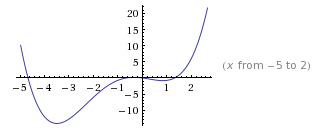
\includegraphics[width=0.40\textwidth]{images/wu2_plot.png}
	\caption{Plot}
	\label{fig:wu2_plot}
\end{figure}


$f(x) = 0.25x^4 + x^3 - x^2 - x$

$f'(x) = x^3 + 3x^2 - 2x - 1$

The global minimum of the function is at $x \approx -3.49086$ and the local minimum at $x \approx 0.83424$
For both runs we use a stepsize of $0.2$ and $100$ iterations. 

1. Local minimum with start at $x = 1$:
x, trajectory = gd.gd(lambda x: ((1/4)*pow(x,4) + pow(x,3) - pow(x,2) - x), lambda x: (pow(x,3)+3*pow(x,2)-2*x-1), 1, 100, 0.2)

2. Global minimum with start at $x = 2$:
x, trajectory = gd.gd(lambda x: ((1/4)*pow(x,4) + pow(x,3) - pow(x,2) - x), lambda x: (pow(x,3)+3*pow(x,2)-2*x-1), 1, 100, 0.2)


\section{WU3}
N/A
